\documentclass{article}
\usepackage{graphicx}
\usepackage[brazilian]{babel}
\usepackage[utf8]{inputenc}
\usepackage[T1]{fontenc}
\usepackage{amsmath}
\usepackage{amssymb}
\setlength{\parindent}{0in}

\begin{document}
	
	\title{Provinha 02 - MAE0119}
	\author{Daniel Yoshio Hotta – 9922700}
	
	\begin{figure}[h]
		\caption{Exercício}
		\centering % para centralizarmos a figura
		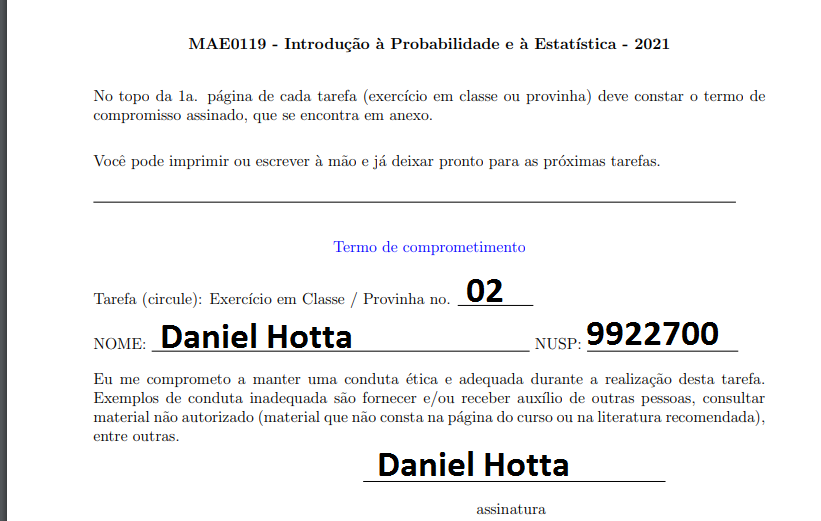
\includegraphics[width=14cm]{termo.png} % leia abaixo
		\label{figura: Termo}
	\end{figure}
	
	\maketitle	
	
	\textbf {E.a} 
	\\ \\
	\textit {Resposta:} \\
    
    Temos $10^7$ formas de os passageiros descerem, uma vez que cada passageiro pode 'escolher' 10 andares para descer, como temos 7 passageiros, temos $10 * 10 * ... * 10 = 10^7$\\
    
    \maketitle	
    
    \textbf {E.b} 
    \\ \\
    \textit {Resposta:} \\
	
    Temos $10 * 9 * 8 * .... * 4$ possibilidades, uma vez que o primeiro passageiro pode escolher 10 andares para descer, o segundo, pode escolher 9, já que não pode descer no mesmo andar que o anterior, o terceiro, só pode 8, porque os outros 2 já foram ocupados e assim por diante.\\
	
\end{document}
